\documentclass{gunote}
% preamble
\usepackage{tikz}
\usetikzlibrary{arrows.meta, decorations}
\usepackage{amsmath, tabularray, hyperref}
\newminted{latex}{rulecolor=mahiropink2}
\newminted{cpp}{rulecolor=mahirodark}
\newminted{python}{rulecolor=asahigreen}
\newminted{text}{rulecolor=asahibrown}
\title{gunote \LaTeX{}笔记模板}
\author{Gemini Usagi,School of Geodesy and Geodetic,Wuhan University}
\date{\today}

\newcommand{\cmd}[1]{\texttt{\backslash #1}}
\def\mbi{\symbfit}
\def\mbu{\symbfup}
% main
\begin{document}
\maketitle
\tableofcontents
\chapter{章节测试}
\section{字体测试}
\textsf{gunote}模板为自用模板,基于\textsf{fontspec}宏包、\textsf{unicode-math}宏包和\textsf{ctex}宏包进行了自定义的字体设置。
\subsection{英文字体}
英文字体设置,罗马字族设置为TeX Gyre Pagella,该字体大多数\TeX{}Live发行版的用户应该都有,在命令行中输入
\begin{Code*}[text]
fc-match -v 'TeX Gyre Pagella'
\end{Code*}
可以查看自己是否拥有字体,以及字体所在的路径。
\begin{Code*}[latex]
\setmainfont{TeX Gyre Pagella}
\end{Code*}
由于TeX Gyre Pagella字体具有\texttt{-regular}、\texttt{-bold}、\texttt{-italic}和\texttt{-bolditalic}的设计,因此使用命令
\begin{Code*}[latex]
\textbf{some text}
\textit{some text}
{\bfseries\itshape some text}
\end{Code*}
可以分别得到如下的效果:\textbf{some text}\quad\textit{some text}\quad{\bfseries\itshape some text}.

无衬线字族设置为\textsf{Gill Sans MT},打字机字族设置为\texttt{JetBrains Mono},前者为Windows平台下的默认字体,后者为JetBrains公司开发的免费开源字体\footnote{下载网址:\url{https://www.jetbrains.com/zh-cn/lp/mono/}}。
\subsection{数学字体}
通过\textsf{unicode-math}宏包提供的\cmd{setmathfont}命令可以很方便地设置数学字体,本模板使用的数学字体为TeX Gyre Pagella Math,效果如下:
{
\def\rcv{\mathrm{r}}
\def\sat{\mathrm{s}}
\begin{gather}
  p_{\rcv,j}^\sat=\rho_\rcv^\sat+c(dt_\rcv-dt^\sat)+T_\rcv^\sat+I_{\rcv,j}^\sat+e_{\rcv,j}^\sat,\\
  \varphi_{\rcv,j}^\sat=\rho_\rcv^\sat+c(dt_\rcv-dt^\sat)+T_\rcv^\sat-I_{\rcv,j}^\sat+\lambda_j N_{\rcv,j}^\sat+\varepsilon_{\rcv,j}^\sat.
\end{gather}
}

在矩阵和向量的表示上,作者所在的专业往往采用加粗的方式。得益于\textsf{unicode-math}宏包对数学字体的处理机制,推荐使用\cmd{symbfit}命令得到粗斜数学字体。
\begin{gather}
  \hat{\mbi{x}}_{k\mid k-1}=\mbi{\Phi}_{k\mid k-1}\hat{\mbi{x}}_{k-1},\\
  \hat{\mbi{P}}_{k\mid k-1}=\mbi{\Phi}_{k\mid k-1}\hat{\mbi{P}}_{k-1}\mbi{\Phi}_{k\mid k-1}^\top+\mbi{Q}_k.
\end{gather}
有时习惯采用直立而非倾斜的数学字体,推荐使用\cmd{symbfup}命令
\begin{gather}
  \hat{\mbu{x}}_{k\mid k-1}=\mbu{\Phi}_{k\mid k-1}\hat{\mbu{x}}_{k-1},\\
  \hat{\mbu{P}}_{k\mid k-1}=\mbu{\Phi}_{k\mid k-1}\hat{\mbu{P}}_{k-1}\mbu{\Phi}_{k\mid k-1}^\top+\mbu{Q}_k.
\end{gather}

特别地,对于数学书法体(caligraphy),模板单独采用Latin Modern Math字体:
\begin{equation}
  \symcal{P}_{\symup{HMI}}=\symcal{P}\left(\vert x-\hat{x}\vert>\symup{PL},\vert q\vert<T\right).
\end{equation}
\subsection{中文字体}
中文字体通过\textsf{ctex}宏包对\textsf{xeCJK}宏包内容的调用,以及预定义的一些命令,实现自定义中文字体。通过输入
\begin{Code*}[latex]
\LoadClass[fontset=none]{ctexrep}
\end{Code*}
实现对\textsf{ctex}宏包的调用,同时声明自定义字体。中文默认宋体字族为思源宋体Source Han Serif CN,黑体字族为苹方字体.PingFang SC,楷体字族为系统默认楷体KaiTi.

文中的很多场合需要用到加粗的文字来表示强调,此时推荐使用
\begin{Code*}[latex]
\textbf{强调文字}
\end{Code*}
来实现,效果:\textbf{强调文字}。此时使用的是思源宋体的Bold样式。

如果习惯于Word那样黑体加粗的格式,可以使用
\begin{Code*}[latex]
{\bfseries\sffamily 黑体加粗}
% 或者
\textbf{\heiti 黑体加粗}
\end{Code*}
来实现,效果:{\bfseries\sffamily 黑体加粗}。此时使用的是苹方字体的Medium样式。
\subsection{日文字体}
作者并不了解\LaTeX{}日文排版或是多语言混合排版的相关领域,暂且只将平假名和片假名罗列至此。
\begin{table}[ht]
  \centering
  \caption{\label{tab:hiragana} 平假名一览}
  \begin{tblr}{colspec=cccccccccccc}
    \hline
    \textbf{ん}行 & \textbf{わ}行 & \textbf{ら}行 & \textbf{や}行 & \textbf{ま}行 & \textbf{は}行 & \textbf{な}行 & \textbf{た}行 & \textbf{さ}行 & \textbf{か}行 & \textbf{あ}行 & \\
    \hline
    ん & わ & ら & や & ま & は & な & た & さ & か & あ & あ段 \\
    \hline
     &  & り &  & み & ひ & に & ち & し & き & い & い段 \\
    \hline
     &  & る & ゆ & む & ふ & ぬ & つ & す & く & う & う段 \\
    \hline
     &  & れ &  & め & へ & ね & て & せ & け & え & え段 \\
    \hline
     & を & ろ & よ & も & ほ & の & と & そ & こ & お & お段 \\
    \hline 
  \end{tblr}
\end{table}
\begin{table}[ht]
  \centering
  \caption{\label{tab:katakana} 片假名一览}
  \begin{tblr}{colspec=cccccccccccc}
    \hline
    \textbf{ン}行 & \textbf{ワ}行 & \textbf{ラ}行 & \textbf{ヤ}行 & \textbf{マ}行 & \textbf{ハ}行 & \textbf{ナ}行 & \textbf{タ}行 & \textbf{サ}行 & \textbf{カ}行 & \textbf{ア}行 & \\
    \hline
    ン & ワ & ラ & ヤ & マ & ハ & ナ & タ & サ & カ & ア & ア段 \\
    \hline
     &  & リ &  & ミ & ヒ & ニ & チ & シ & キ & イ & イ段 \\
    \hline
     &  & ル & ユ & ム & フ & ヌ & ツ & ス & ク & ウ & ウ段 \\
    \hline
     &  & レ &  & メ & ヘ & ヌ & テ & セ & ケ & エ & エ段 \\
    \hline
     & ヲ & ロ & ヨ & モ & ホ & ノ & ト & ソ & コ & オ & オ段 \\
    \hline 
  \end{tblr}
\end{table}
\section{颜色测试}
作者基于\textsf{xcolor}宏包,参考Onimai Character\footnote{\url{https://onimai.jp/character/}}设计了部分颜色,并定义了一些颜色命令,如果你希望在文档中使用这些颜色,请参照表\ref{tab:color},将角色的假名部分罗马音和名称叠加,就可以拿到预览效果中的颜色,或者直接根据RGB值进行颜色的自定义。
\begin{table}[htbp]
  \centering
  \caption{\label{tab:color} 预定义颜色}
  \begin{tblr}{
    colspec={cccc|cccc},
    cell{2}{1}={r=5}{c},
    cell{2}{3}={mahirolight},
    cell{3}{3}={mahirodark},
    cell{4}{3}={mahiropink1},
    cell{5}{3}={mahiropink2},
    cell{6}{3}={mahirogray},
    cell{3}{5}={r=3}{c},
    cell{3}{7}={miharigold},
    cell{4}{7}={miharipurple},
    cell{5}{7}={miharired},
    cell{7}{1}={r=2}{c},
    cell{7}{3}={momijibrown},
    cell{8}{3}={momijiblue},
    cell{7}{5}={r=2}{c},
    cell{7}{7}={kaedepink},
    cell{8}{7}={kaedeblue},
    cell{9}{1}={r=2}{c},
    cell{9}{3}={asahibrown},
    cell{10}{3}={asahigreen},
    cell{9}{5}={r=2}{c},
    cell{9}{7}={miyopurple},
    cell{10}{7}={miyoyellow}
  }
    \hline
    取材角色 & 名称 & 预览 & RGB值 & 取材角色 & 名称 & 预览 & RGB值 \\
    \hline
    緒山まひろ & light &  & 228,243,248 &  &  &  &  \\
     & gray &  & 133,149,174 & 緒山みはり & gold &  & 245,195,134 \\
     & pink1 &  & 234,157,169 &  & purple &  & 221,157,240 \\
     & pink2 &  & 234,212,207 &  & red &  & 234,140,156 \\
     & dark &  & 125,134,156 &  &  &  &  \\
    \hline 
    穂月もみじ & brown &  & 151,119,128 & 穂月かえで & pink &  & 241,172,184 \\
     & blue &  & 152,213,238 &  & blue &  & 103,210,231 \\
    \hline
    桜花あさひ & brown &  & 188,153,134 & 室崎みよ & purple &  & 185,133,145 \\
     & green &  & 119,147,109 &  & yellow &  & 254,234,153 \\
    \hline
  \end{tblr}
\end{table}
部分颜色被有机地穿插进了文档的各个元素中。
\section{自定义环境测试}
\subsection{定理类环境}
模板基于\textsf{tcolorbox}宏包定义了下面的定理类环境。
\subsubsection{Example环境}
样例如下:
\begin{Example}[halign lower=flush center, sidebyside]{单位复数群}{S1}
  第一个李群的例子,是最便于可视化的,在复数乘法下的单位复数。单位复数有着$\symbf{z}=\cos\theta+i\sin\theta$的形式。

  如图所示的$S^1$流形是一个复平面$\symbb{C}$上的单位圆,流形上存在着单位复数$\symbf{z}^*\symbf{z}=1$.李代数$\symfrak{s}^1=T_{\symcal{E}}S^1$是虚轴$i\symbb{R}$(标红),任何切空间$TS^1$都是直线$\symbb{R}$的同构。切向量(红色部分)所包围的流形对应了一段圆弧(蓝色部分)。
  \tcblower
  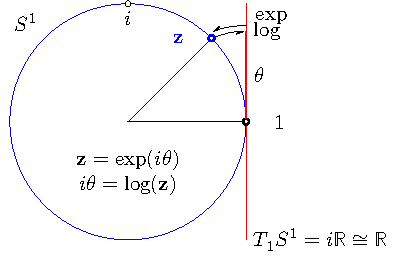
\includegraphics{picture/manifold.pdf}
\end{Example}
\subsubsection{Definition环境}
样例如下:
\begin{Definition}{数域}{field}
  设 $\symbb{K}$ 是复数集 $\symbb{C}$ 的子集且至少有两个不同的元素,如果 $\symbb{K}$ 中任意两个数的加法、减法、乘法和除法(除数不为零)仍属于 $\symbb{K}$ ,则称 $\symbb{K}$ 是一个数域。
\end{Definition}
\subsubsection{Theorem环境}
样例如下:
\begin{Theorem}{}{number field}
  任一数域必包含有理数域 $\symbb{Q}$ .
\end{Theorem}
\subsubsection{Proof环境和QED符号}
\textsf{Proof}环境比较灵活,由下面的定义得到:
\begin{Code*}[latex]
\newcommand{\QEDsymbol}{\hfill$\square$}
\newenvironment{Proof}{\textbf{证:}}{\QEDsymbol} % Proof env
\end{Code*}
因此该环境不进行换行。除此之外,模板还提供了 \textsf{\backslash QEDsymbol} 命令表示证毕符号。样例如下:

\begin{Proof}
  由上面知道,$1$ 必属于任一数域。将 $1$ 连加 $n$ 次,则 $n$ 也应属于该属于,因此任一正整数属于该数域。又 $0-n=-n$ ,因此 $-n$ 也应在此数域中。因而整数全体都必须在这个数域之中。最后,若 $m\neq 0$,\ $m$,\ $n$ 为整数,则由除法封闭性可知 $\frac{n}{m}$ 也应属于该数域,即任一有理数都应在此数域中。
\end{Proof}
\subsection{代码环境}
模板基于\textsf{tcolorbox}宏包和\textsf{minted}宏包定义了下面的代码环境\textsf{Code},效果如下:
\begin{Code}{test.tex}
\begin{tikzpicture}
  \node (A) at (0,0) {};
  \draw[red] (A) -- (1,0);
\end{tikzpicture}
\end{Code}

该环境包含一个必须参数和一个可选参数,其中必须参数为标题,可选参数为编程语言。此外,模板还单独定义了\textsf{Code*}环境,该环境不进行编号,也不输出标题,因此只有一个可选参数。
\begin{Code*}[cpp]
#include <iostream>
using namespace std;

int main() {
  cout << "测试" << endl;
}
\end{Code*}
\end{document}